% Options for packages loaded elsewhere
\PassOptionsToPackage{unicode}{hyperref}
\PassOptionsToPackage{hyphens}{url}
%
\documentclass[
]{book}
\usepackage{amsmath,amssymb}
\usepackage{lmodern}
\usepackage{iftex}
\ifPDFTeX
  \usepackage[T1]{fontenc}
  \usepackage[utf8]{inputenc}
  \usepackage{textcomp} % provide euro and other symbols
\else % if luatex or xetex
  \usepackage{unicode-math}
  \defaultfontfeatures{Scale=MatchLowercase}
  \defaultfontfeatures[\rmfamily]{Ligatures=TeX,Scale=1}
\fi
% Use upquote if available, for straight quotes in verbatim environments
\IfFileExists{upquote.sty}{\usepackage{upquote}}{}
\IfFileExists{microtype.sty}{% use microtype if available
  \usepackage[]{microtype}
  \UseMicrotypeSet[protrusion]{basicmath} % disable protrusion for tt fonts
}{}
\makeatletter
\@ifundefined{KOMAClassName}{% if non-KOMA class
  \IfFileExists{parskip.sty}{%
    \usepackage{parskip}
  }{% else
    \setlength{\parindent}{0pt}
    \setlength{\parskip}{6pt plus 2pt minus 1pt}}
}{% if KOMA class
  \KOMAoptions{parskip=half}}
\makeatother
\usepackage{xcolor}
\usepackage{color}
\usepackage{fancyvrb}
\newcommand{\VerbBar}{|}
\newcommand{\VERB}{\Verb[commandchars=\\\{\}]}
\DefineVerbatimEnvironment{Highlighting}{Verbatim}{commandchars=\\\{\}}
% Add ',fontsize=\small' for more characters per line
\usepackage{framed}
\definecolor{shadecolor}{RGB}{248,248,248}
\newenvironment{Shaded}{\begin{snugshade}}{\end{snugshade}}
\newcommand{\AlertTok}[1]{\textcolor[rgb]{0.94,0.16,0.16}{#1}}
\newcommand{\AnnotationTok}[1]{\textcolor[rgb]{0.56,0.35,0.01}{\textbf{\textit{#1}}}}
\newcommand{\AttributeTok}[1]{\textcolor[rgb]{0.77,0.63,0.00}{#1}}
\newcommand{\BaseNTok}[1]{\textcolor[rgb]{0.00,0.00,0.81}{#1}}
\newcommand{\BuiltInTok}[1]{#1}
\newcommand{\CharTok}[1]{\textcolor[rgb]{0.31,0.60,0.02}{#1}}
\newcommand{\CommentTok}[1]{\textcolor[rgb]{0.56,0.35,0.01}{\textit{#1}}}
\newcommand{\CommentVarTok}[1]{\textcolor[rgb]{0.56,0.35,0.01}{\textbf{\textit{#1}}}}
\newcommand{\ConstantTok}[1]{\textcolor[rgb]{0.00,0.00,0.00}{#1}}
\newcommand{\ControlFlowTok}[1]{\textcolor[rgb]{0.13,0.29,0.53}{\textbf{#1}}}
\newcommand{\DataTypeTok}[1]{\textcolor[rgb]{0.13,0.29,0.53}{#1}}
\newcommand{\DecValTok}[1]{\textcolor[rgb]{0.00,0.00,0.81}{#1}}
\newcommand{\DocumentationTok}[1]{\textcolor[rgb]{0.56,0.35,0.01}{\textbf{\textit{#1}}}}
\newcommand{\ErrorTok}[1]{\textcolor[rgb]{0.64,0.00,0.00}{\textbf{#1}}}
\newcommand{\ExtensionTok}[1]{#1}
\newcommand{\FloatTok}[1]{\textcolor[rgb]{0.00,0.00,0.81}{#1}}
\newcommand{\FunctionTok}[1]{\textcolor[rgb]{0.00,0.00,0.00}{#1}}
\newcommand{\ImportTok}[1]{#1}
\newcommand{\InformationTok}[1]{\textcolor[rgb]{0.56,0.35,0.01}{\textbf{\textit{#1}}}}
\newcommand{\KeywordTok}[1]{\textcolor[rgb]{0.13,0.29,0.53}{\textbf{#1}}}
\newcommand{\NormalTok}[1]{#1}
\newcommand{\OperatorTok}[1]{\textcolor[rgb]{0.81,0.36,0.00}{\textbf{#1}}}
\newcommand{\OtherTok}[1]{\textcolor[rgb]{0.56,0.35,0.01}{#1}}
\newcommand{\PreprocessorTok}[1]{\textcolor[rgb]{0.56,0.35,0.01}{\textit{#1}}}
\newcommand{\RegionMarkerTok}[1]{#1}
\newcommand{\SpecialCharTok}[1]{\textcolor[rgb]{0.00,0.00,0.00}{#1}}
\newcommand{\SpecialStringTok}[1]{\textcolor[rgb]{0.31,0.60,0.02}{#1}}
\newcommand{\StringTok}[1]{\textcolor[rgb]{0.31,0.60,0.02}{#1}}
\newcommand{\VariableTok}[1]{\textcolor[rgb]{0.00,0.00,0.00}{#1}}
\newcommand{\VerbatimStringTok}[1]{\textcolor[rgb]{0.31,0.60,0.02}{#1}}
\newcommand{\WarningTok}[1]{\textcolor[rgb]{0.56,0.35,0.01}{\textbf{\textit{#1}}}}
\usepackage{longtable,booktabs,array}
\usepackage{calc} % for calculating minipage widths
% Correct order of tables after \paragraph or \subparagraph
\usepackage{etoolbox}
\makeatletter
\patchcmd\longtable{\par}{\if@noskipsec\mbox{}\fi\par}{}{}
\makeatother
% Allow footnotes in longtable head/foot
\IfFileExists{footnotehyper.sty}{\usepackage{footnotehyper}}{\usepackage{footnote}}
\makesavenoteenv{longtable}
\usepackage{graphicx}
\makeatletter
\def\maxwidth{\ifdim\Gin@nat@width>\linewidth\linewidth\else\Gin@nat@width\fi}
\def\maxheight{\ifdim\Gin@nat@height>\textheight\textheight\else\Gin@nat@height\fi}
\makeatother
% Scale images if necessary, so that they will not overflow the page
% margins by default, and it is still possible to overwrite the defaults
% using explicit options in \includegraphics[width, height, ...]{}
\setkeys{Gin}{width=\maxwidth,height=\maxheight,keepaspectratio}
% Set default figure placement to htbp
\makeatletter
\def\fps@figure{htbp}
\makeatother
\setlength{\emergencystretch}{3em} % prevent overfull lines
\providecommand{\tightlist}{%
  \setlength{\itemsep}{0pt}\setlength{\parskip}{0pt}}
\setcounter{secnumdepth}{5}
\usepackage{booktabs}
\ifLuaTeX
  \usepackage{selnolig}  % disable illegal ligatures
\fi
\usepackage[]{natbib}
\bibliographystyle{plainnat}
\IfFileExists{bookmark.sty}{\usepackage{bookmark}}{\usepackage{hyperref}}
\IfFileExists{xurl.sty}{\usepackage{xurl}}{} % add URL line breaks if available
\urlstyle{same} % disable monospaced font for URLs
\hypersetup{
  pdftitle={SDMX Constructor: User Manual},
  pdfauthor={International Labour Organization: Department of Statistics},
  hidelinks,
  pdfcreator={LaTeX via pandoc}}

\title{SDMX Constructor: User Manual}
\author{International Labour Organization: Department of Statistics}
\date{2023-04-25}

\usepackage{amsthm}
\newtheorem{theorem}{Theorem}[chapter]
\newtheorem{lemma}{Lemma}[chapter]
\newtheorem{corollary}{Corollary}[chapter]
\newtheorem{proposition}{Proposition}[chapter]
\newtheorem{conjecture}{Conjecture}[chapter]
\theoremstyle{definition}
\newtheorem{definition}{Definition}[chapter]
\theoremstyle{definition}
\newtheorem{example}{Example}[chapter]
\theoremstyle{definition}
\newtheorem{exercise}{Exercise}[chapter]
\theoremstyle{definition}
\newtheorem{hypothesis}{Hypothesis}[chapter]
\theoremstyle{remark}
\newtheorem*{remark}{Remark}
\newtheorem*{solution}{Solution}
\begin{document}
\maketitle

{
\setcounter{tocdepth}{1}
\tableofcontents
}
\hypertarget{preface}{%
\chapter*{Preface}\label{preface}}
\addcontentsline{toc}{chapter}{Preface}

Welcome to the \textbf{SDMX Constructor User Manual!}

SDMX Constructor\footnote{It was previously called DSD Constructor, it supported creating and editing Data Structure Definitions (DSDs) and their related artefacts (i.e., concept schemes and code lists). The significant improvements and additions to the software justify the name change of the tool from DSD Constructor to SDMX Constructor. With the latest update, the tool can now translate SDMX artefacts in multiple languages, integrate with the .Stat Suite, and manage reference metadata. Additionally, the tool now includes Table Modeller functionalities that make it easier for users who are new to SDMX to understand and use the software. The updated software is no longer just a DSD Constructor but a complete SDMX Constructor capable of handling various aspects of SDMX data and metadata. The new name better reflects the software's expanded capabilities, making it more relevant and recognizable to the target audience (\url{https://ilostat.github.io/dsdc/}).} is a powerful desktop software tool that helps users model aggregate data per the SDMX standards \footnote{An ISO standard (since 2005, version 2.1 since 2013): \url{https://www.iso.org/obp/ui/fr/\#iso:std:iso:17369:ed-1:v1:en} and \url{https://sdmx.org/?page_id=5008}} . It eases generating and editing SDMX artefacts and ultimately supports data availability and access through SDMX-compliant data portals (such as ones built with .Stat Suite\footnote{To learn more about the .Stat Suite platform please refer to the documentation here: \url{https://siscc.org/stat-suite/}. The SDMX Constructor has been optimised to seamlessly integrate with the .Stat Suite platform, as its back-end client.} ).

SDMX Constructor is one of the tools that comprise the ILO SDMX toolkit \footnote{\url{https://ilostat.ilo.org/resources/sdmx-tools/}}, alongside SMART (Statistical Metadata-driven Analysis and Reporting Tool) and the SDMX Excel Add-in.

This user manual for the SDMX Constructor provides step-by-step instructions on using the tool in a user-friendly and accessible manner. It provides an in-depth understanding of SDMX Constructor's features and functionalities. It is an essential resource for anyone using the tool to manage and share data following the SDMX standards.

Below is a screenshot of the tool's landing page as an example of the user interface.

\begin{figure}

{\centering 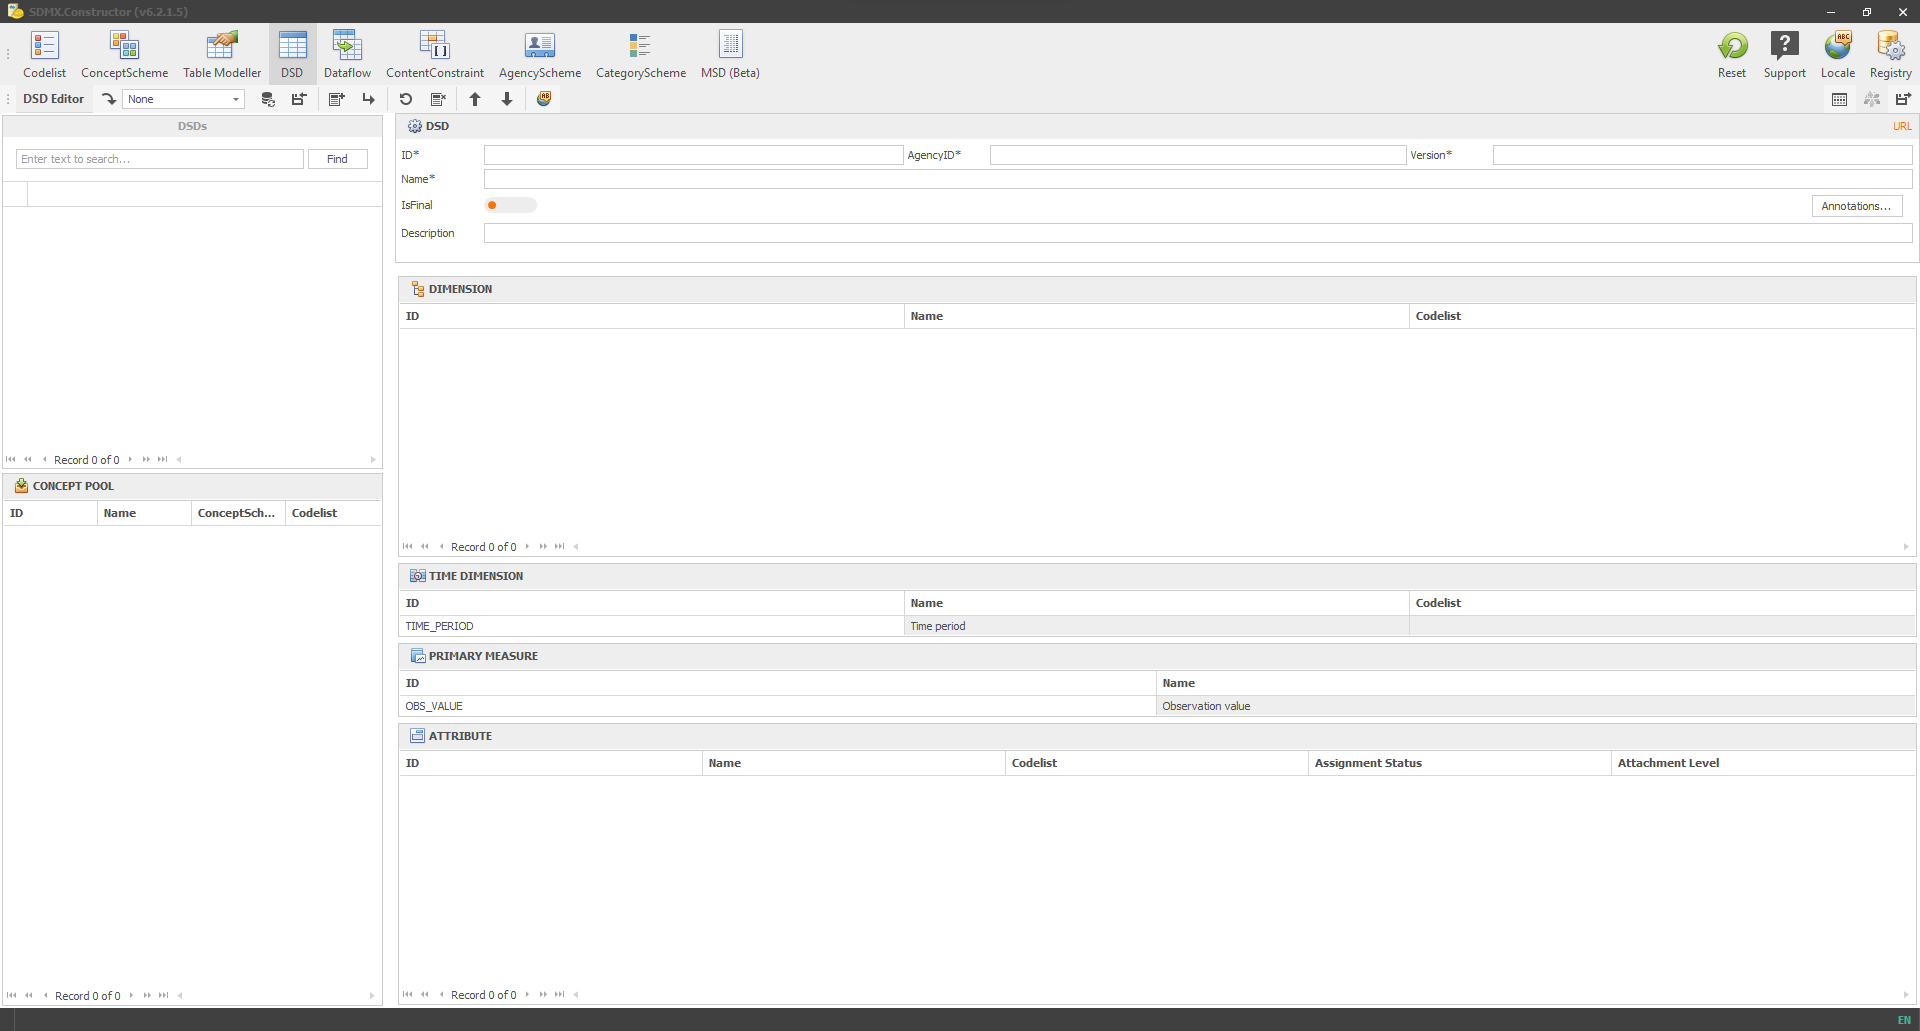
\includegraphics[width=1\linewidth]{./images/image001} 

}

\caption{A screenshot of SDMX Constructor}\label{fig:front-cover}
\end{figure}

\href{images/image001.png}{Click here to enlarge the image}

\hypertarget{audience-and-use-cases}{%
\section*{Audience and use cases}\label{audience-and-use-cases}}
\addcontentsline{toc}{section}{Audience and use cases}

The SDMX Constructor is designed to meet the needs of a wide range of users, from beginners who are new to SDMX to data managers who need advanced capabilities for managing large and complex datasets. In addition to these user types, there may be other groups of users with specific requirements or use cases. This user manual provides guidance and instructions for using the SDMX Constructor, focusing on the needs of these various user types.

\textbf{SDMX beginners}: These users are new to SDMX and want to use the SDMX Constructor to view, edit, and create new SDMX structural artefacts. They may need assistance understanding the SDMX concepts, terminology, and the software's user interface.

For SDMX beginners, this manual explains using the SDMX Constructor to access, view, edit, and create SDMX structural artefacts from SDMX registries. While one can find information on SDMX concepts and terminology from other sources, this manual focuses explicitly on the user interfaces of the SDMX Constructor. The SDMX beginners may be keen to know how to \protect\hyperlink{accessing-sdmx}{access SDMX artefacts from default SDMX registries} and \protect\hyperlink{connect-to}{connect to a new SDMX registry} from the SDMX Constructor.

\textbf{Data managers}: These users are likely familiar with the SDMX concepts and terminology and may require information about advanced functionalities offered by the SDMX Constructor. For example, they may want to use the SDMX Constructor as a backend client to manage SDMX artefacts for the .Stat Data Lifecycle Manager (DLM). For such cases, they may also use the SDMX Constructor to build the initial structural metadata when creating a new .Stat Suite instance.

There are several topics that data managers may be interested in learning when it comes to \protect\hyperlink{creating-sdmx}{creating SDMX artefacts from scratch}. Firstly, they may want to start by \protect\hyperlink{setting-up}{setting up a registry as a local folder}. Next, they can \protect\hyperlink{preparing-inputs}{prepare inputs} and create several artefacts, including the \protect\hyperlink{creating-agencyschme}{AgencyScheme}, \protect\hyperlink{creating-conceptscheme}{ConceptScheme, and Codelist} and the \protect\hyperlink{creating-dsd}{DSD, Dataflow, ContentConstraint, and CategoryScheme}. After creating these artefacts, they may want to learn how to \protect\hyperlink{upload-the}{upload the XML file to the Data Lifecycle Manager (DLM)}. Additionally, they may want to know how to \protect\hyperlink{access-sdmx}{access SDMX artefacts from default SDMX registries} and \protect\hyperlink{connect-to}{connect to a new SDMX registry} for editing SDMX artefacts directly in the DLM.

\textbf{SDMX metadata managers}: These users manage SDMX artefacts and ensure their accuracy and consistency. They may use the SDMX Constructor to model data and modify SDMX structural artefacts, including translating SDMX artefacts in various languages, managing annotations and creating Metadata Structure Definition (MSD).

\hypertarget{scope-and-assumptions}{%
\section*{Scope and assumptions}\label{scope-and-assumptions}}
\addcontentsline{toc}{section}{Scope and assumptions}

This comprehensive manual provides a step-by-step guide on getting started with the software, including installing it and creating and managing SDMX artefacts. The manual includes a detailed overview of the tool's user interfaces, including menu items, navigation, and other essential features. The manual does not, however, delve into the intricacies of the SDMX standard itself. Describing the SDMX standard is beyond the scope of this manual, as it is an extensive and complex topic requiring more in-depth discussion and is available elsewhere. Instead, the manual assumes that readers are familiar with the SDMX standard and focuses on explaining how to use the tool within that context.

\hypertarget{overview}{%
\section*{Overview}\label{overview}}
\addcontentsline{toc}{section}{Overview}

The chapters in this manual build up toward providing comprehensive guidance that covers topics users need to know to get started with the application, understand its navigation, and use its features and functionalities to model data effectively. The manual includes the following chapters.

\begin{itemize}
\tightlist
\item
  Chapter 1: \protect\hyperlink{benefits-of}{Benefits of SDMX Constructor}
\item
  Chapter 2: \protect\hyperlink{getting-started}{Getting started}
\item
  Chapter 3: \protect\hyperlink{user-interface}{User interface}
\item
  Chapter 4: \protect\hyperlink{using-sdmx}{Using SDMX Constructor}
\item
  Chapter 5: \protect\hyperlink{special-topics}{Special Topics}
\item
  Chapter 6: \protect\hyperlink{glossary}{Glossary}
\end{itemize}

\hypertarget{contact-information}{%
\section*{Contact information}\label{contact-information}}
\addcontentsline{toc}{section}{Contact information}

For more information and to seek basic technical assistance or support on the tool, please reach out International Labour Organization - Department of Statistics at \href{mailto:sdmx.support@ilo.org}{\nolinkurl{sdmx.support@ilo.org}}.

\hypertarget{benefits-of}{%
\chapter{Benefits of SDMX Constructor}\label{benefits-of}}

SDMX Constructor is a software tool that offers a range of features and functionalities designed to streamline and optimise the SDMX workflow, making it an essential tool for statistical organisations, data providers, and other stakeholders involved in the production and dissemination of statistical data.

One of the key benefits of SDMX Constructor is that it allows users to access and query SDMX structural artefacts from publicly available SDMX registries (through APIs in the background) in a desktop environment. This makes it easy for users to quickly and easily search for and view essential components of SDMX structural metadata, such as Data Structure Definitions (DSDs) and dataflows.

In addition to its API capabilities, SDMX Constructor offers two other essential features. The first is that it helps users model data following the SDMX standards. For example, SDMX Constructor makes it easy for users to define data structures and create data flows following SDMX standards. This is essential for data providers who need easy-to-use tools to ensure that their data can be shared and used by others in a consistent and standardised way.

The second essential feature of SDMX Constructor is that it enables users to create and edit SDMX artefacts in a user-friendly environment. This includes creating and editing code lists, concept schemes, DSDs, dataflows, content constraints, category schemes and Metadata Structure Definitions (MSDs). SDMX Constructor provides a user-friendly interface that makes it easy for users to create and modify these artefacts without needing to be an expert in SDMX.

Finally, SDMX Constructor supports data availability and access through online data portals. Using SDMX Constructor, data providers can ensure their data is available and accessible through online data portals built on SDMX standards. This allows data users to easily access and use the data they need for their research, analysis, and other activities.

\hypertarget{getting-started}{%
\chapter{Getting Started}\label{getting-started}}

In this chapter, you will find information about the installation process of SDMX Constructor in a Windows environment. Specifically, it will cover the system requirements necessary to install the software, the steps required to download the executable file and the subsequent installation process. The chapter will also explain the software update process, providing practical guidance on keeping your SDMX Constructor current.

\hypertarget{system-requirements}{%
\section{System requirements}\label{system-requirements}}

Before installing any desktop software, ensuring the computer meets the necessary system requirements is essential. These requirements can include hardware specifications like processor speed, memory, and storage capacity, as well as software prerequisites like operating system version and other dependencies. Find below the minimum system requirements for installing and running SDMX Constructor.

\begin{itemize}
\tightlist
\item
  Windows 7 or later in both 32- and 64-bit environments
\item
  .NET 4.5.2 or later with all updates and patches
\item
  200MB disk space for the software
\end{itemize}

\hypertarget{installation}{%
\section{Installation}\label{installation}}

\textbf{Step 1}: Visit the site \url{https://ilostat.github.io/dsdc/} and click on the INSTALL menu option (as shown below).

\begin{center}
\includegraphics[width=1\linewidth]{./images/image003} \end{center}

\textbf{Step 2}: In the resulting page, click on ``here'' (as shown below)

\begin{center}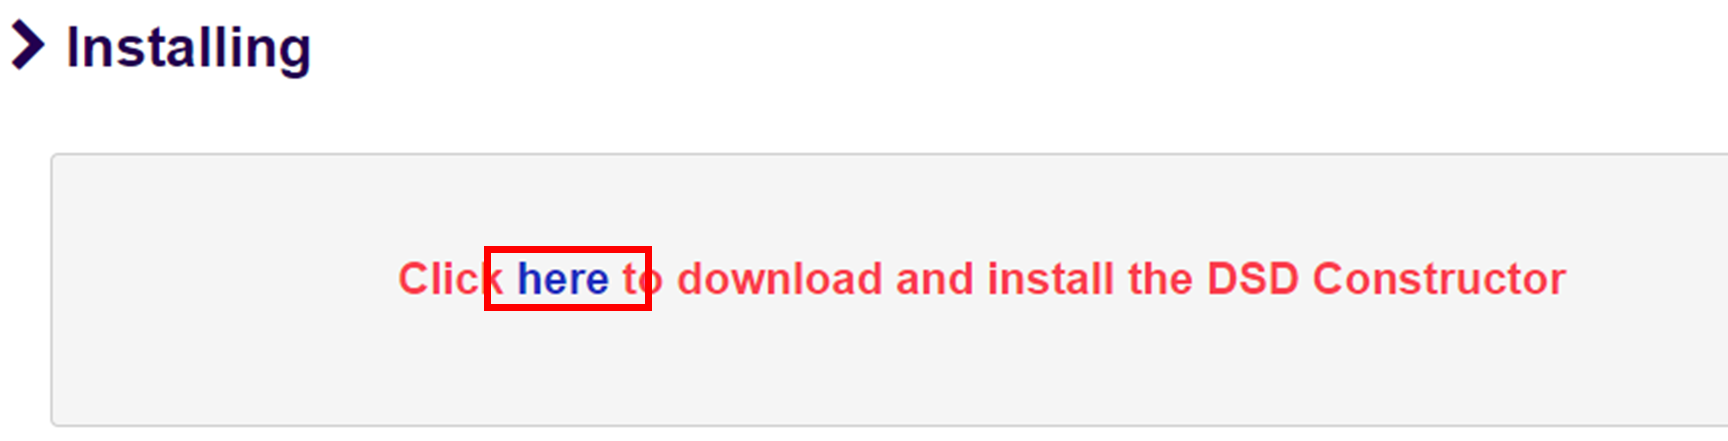
\includegraphics[width=1\linewidth]{./images/image005} \end{center}

\textbf{Step 3}: An interface (as shown below) will open, requiring you to enter a few details (your name, your email, and the name of your organisation (if applicable)).

\begin{center}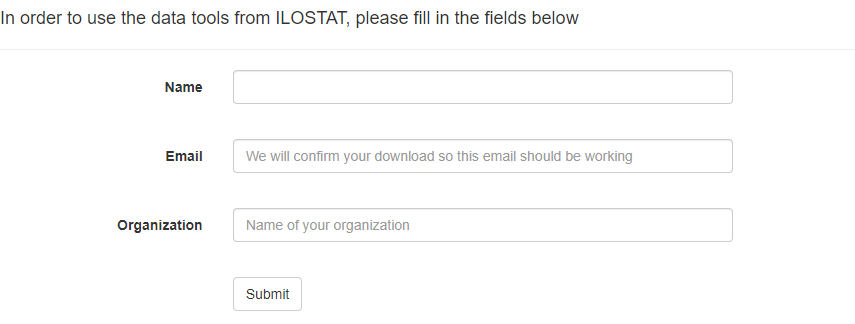
\includegraphics[width=1\linewidth]{./images/image007} \end{center}

\textbf{Step 4}: The download will start when you fill in the form and submit the information. The software installer file, named ``ILOSTAT\_DSD\_Constructor\_Setup.exe'', will be downloaded.

\textbf{Step 5}: Double-click on this file to begin the installation process. Select `Install' on the security message and wait for the installation process to complete.

\hypertarget{software-updates}{%
\section{Software updates}\label{software-updates}}

The SDMX Constructor updates itself to the latest version (if available) using the ClickOnce Deployment technique. This method ensures a streamlined installation process with minimal user involvement. An internet connection is required when launching the application to initiate the update. The software will check for available updates and automatically download and install them in the background without requiring any input from the user. This feature helps to ensure that users always have access to the latest version of the software, with the latest bug fixes, performance improvements, and new features.

\hypertarget{user-interface}{%
\chapter{User Interface}\label{user-interface}}

This chapter will provide you with a comprehensive guide on the main aspects of the SDMX Constructor's user interface. It will cover three main topics. The first topic will be an overview of the user interface, including a detailed explanation of the various menu options, toolbars, and navigation options. The second topic will focus on the inputs and outputs of SDMX Constructor. It will cover the different input options available and the output options. The third topic will provide an overview of the translation functionality in SDMX Constructor.

\hypertarget{interface-overview-and-navigation}{%
\section{Interface overview and navigation}\label{interface-overview-and-navigation}}

The user interface of the tool appears like this:

\begin{center}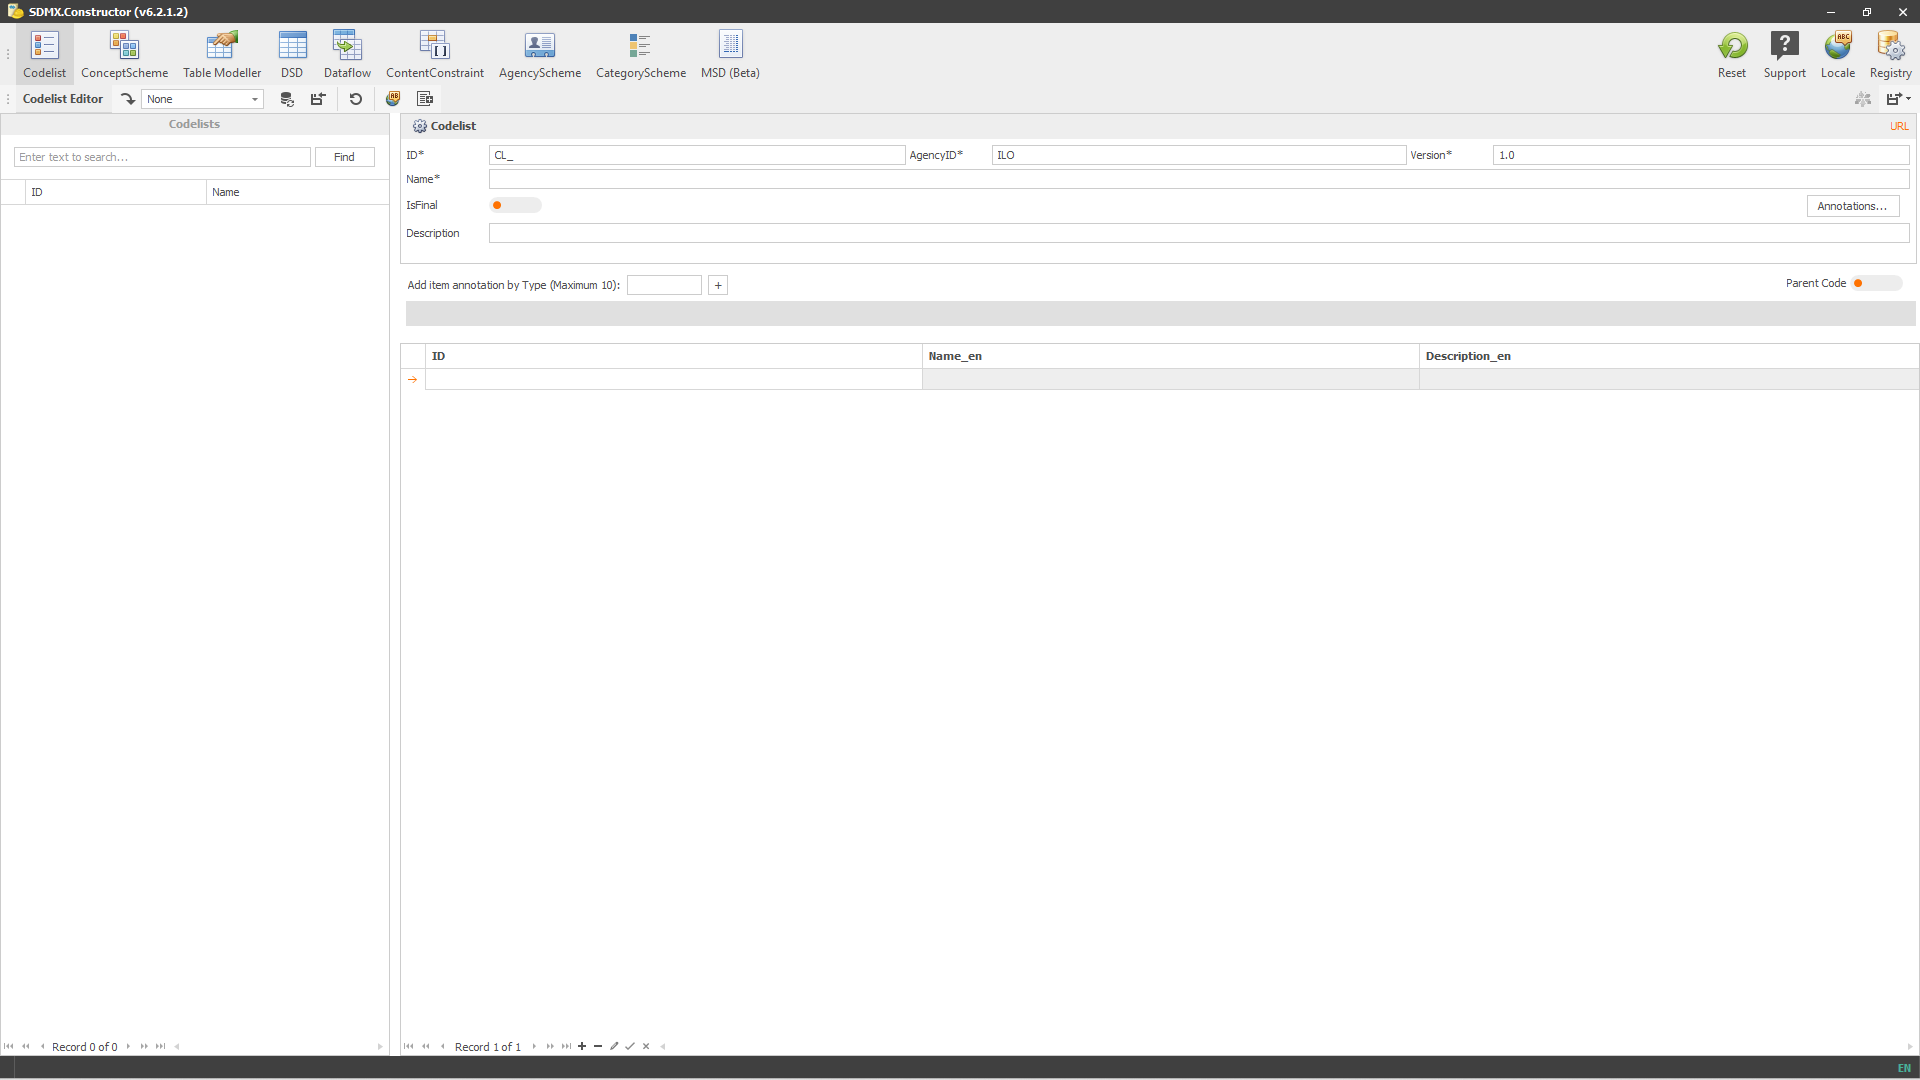
\includegraphics[width=1\linewidth]{./images/image009} \end{center}

\href{images/image009.png}{Click here to enlarge the image}

The interface shows many menu items on top. For example, in the top right corner (as highlighted below), the first group of buttons (General Functions) shows the items applicable to the whole tool. They include Reset, Support, Locale and Registry. See Table 3.1 for a brief overview of the menu items.

\begin{center}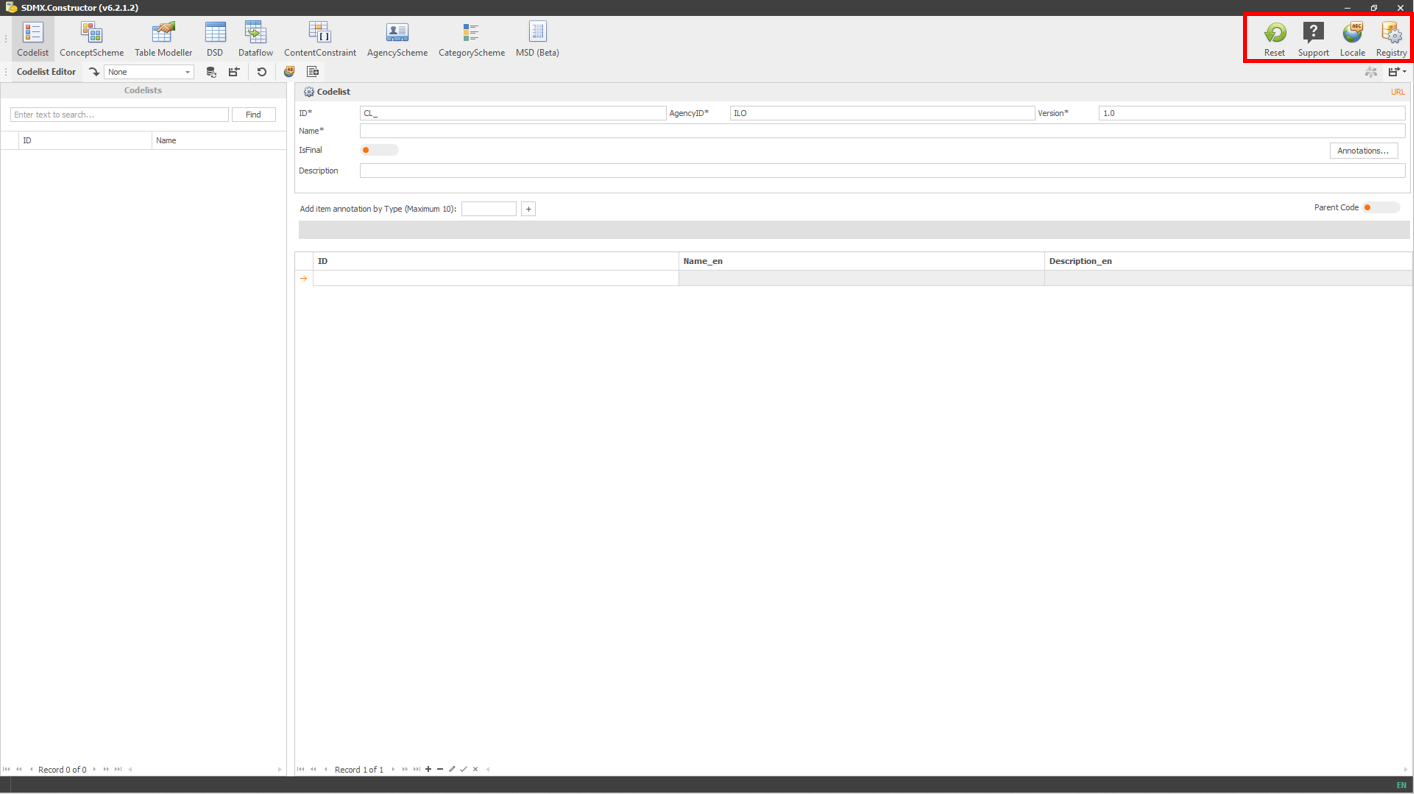
\includegraphics[width=1\linewidth]{./images/image011} \end{center}

\href{images/image011.png}{Click here to enlarge the image}

\begin{longtable}[]{@{}
  >{\raggedright\arraybackslash}p{(\columnwidth - 2\tabcolsep) * \real{0.2676}}
  >{\raggedright\arraybackslash}p{(\columnwidth - 2\tabcolsep) * \real{0.7324}}@{}}
\caption{\label{tab:table31} A bird's-eye view of the menu items in the top right corner (General Functions)}\tabularnewline
\toprule()
\begin{minipage}[b]{\linewidth}\raggedright
Menu item
\end{minipage} & \begin{minipage}[b]{\linewidth}\raggedright
What to expect: A bird's-eye view of General Functions
\end{minipage} \\
\midrule()
\endfirsthead
\toprule()
\begin{minipage}[b]{\linewidth}\raggedright
Menu item
\end{minipage} & \begin{minipage}[b]{\linewidth}\raggedright
What to expect: A bird's-eye view of General Functions
\end{minipage} \\
\midrule()
\endhead
\textbf{Reset} & The Reset button resets the tool to its default settings. It removes all the inputs and initiates a fresh start. \\
\textbf{Support} & The Support button launches the default email application on a computer, with a new email message addressed to the support team for the tool, ready to be composed and sent. \\
\textbf{Locale} & The Support button launches the default email application on a computer, with a new email message addressed to the support team for the tool, ready to be composed and sent. \\
\textbf{Registry} & The Registry button provides several options for users to configure their settings. For example, users can specify the connection details of the SDMX registry (either a local folder or local instance (localhost) or online) and connect with the Data Lifecycle Manager (DLM) component of the .Stat Suite. In addition, the button allows specifying the proxy settings for the internet connection if a proxy is needed. There are also options for entering authentication credentials for automated translation using Google Translation or DeepL API. \\
\bottomrule()
\end{longtable}

The second group of menu items (Editors) shows the options in the top left corner (as highlighted below). They include Codelist, ConceptScheme, Table Modeller, DSD, Dataflow, ConceptConstraint, AgencyScheme, CategoryScheme and MSD. Each menu item is an entry point for creating and editing a specific artefact. Clicking on any of the options will reveal more particular options below. See Table 2 for a brief overview of the menu items (Editors).

\begin{center}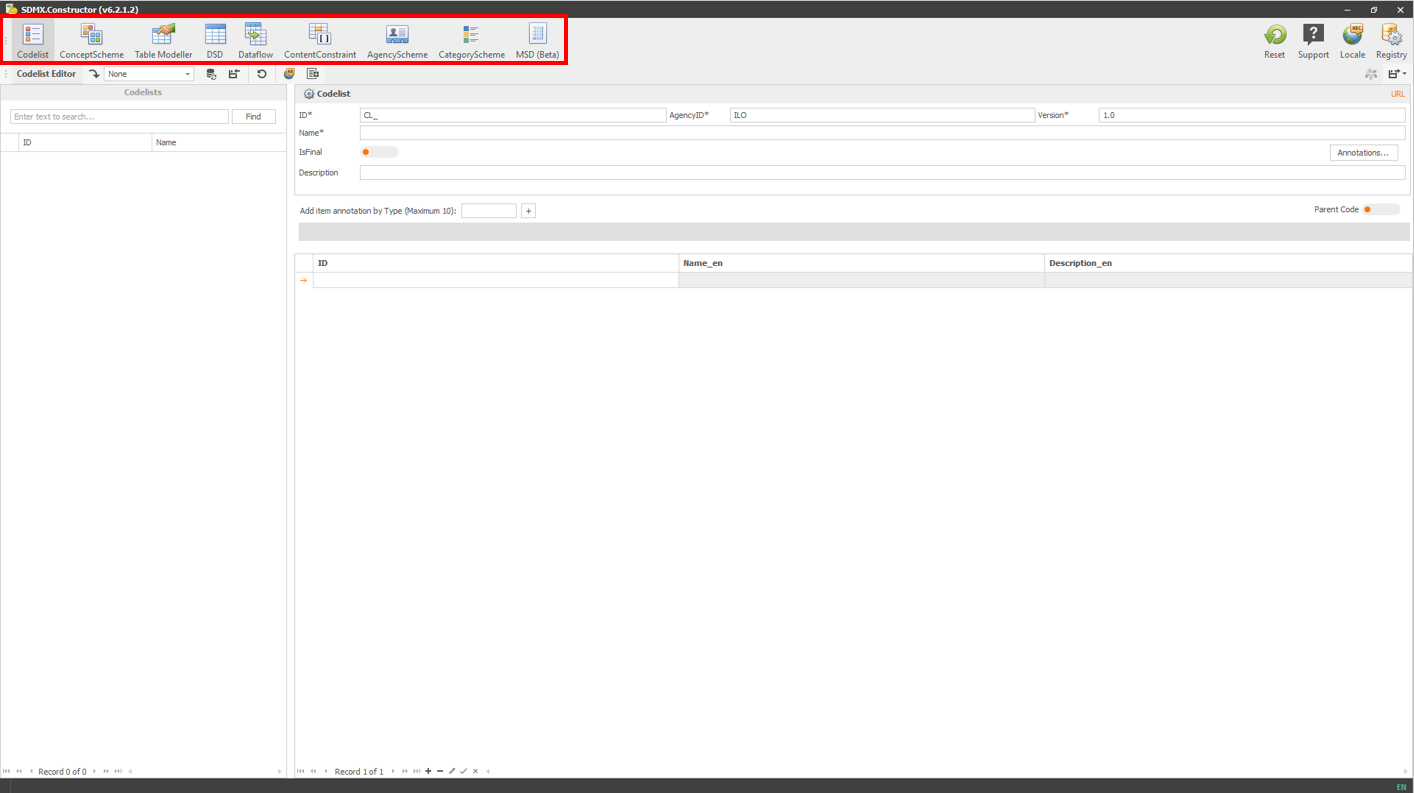
\includegraphics[width=1\linewidth]{./images/image013} \end{center}

\href{images/image013.png}{Click here to enlarge the image}

table

\begin{longtable}[]{@{}
  >{\raggedright\arraybackslash}p{(\columnwidth - 2\tabcolsep) * \real{0.2676}}
  >{\raggedright\arraybackslash}p{(\columnwidth - 2\tabcolsep) * \real{0.7324}}@{}}
\caption{\label{tab:table32} A bird's-eye view of the menu items in the top left corner (Editors)}\tabularnewline
\toprule()
\begin{minipage}[b]{\linewidth}\raggedright
Menu item
\end{minipage} & \begin{minipage}[b]{\linewidth}\raggedright
What to expect: A bird's-eye view of the menu items in the top left corner (Editors)
\end{minipage} \\
\midrule()
\endfirsthead
\toprule()
\begin{minipage}[b]{\linewidth}\raggedright
Menu item
\end{minipage} & \begin{minipage}[b]{\linewidth}\raggedright
What to expect: A bird's-eye view of the menu items in the top left corner (Editors)
\end{minipage} \\
\midrule()
\endhead
\textbf{Codelist} & The Codelist button shows an interface to create or edit the list of Concepts (dimensions/attributes of a modelled dataset), each having a list of possible values or codes. The codes have unique IDs and (multilingual) labels and may have other information such as order and hierarchy. \\
\textbf{ConceptScheme} & The ConceptScheme button shows an interface to create or edit the Concepts (dimensions/attributes of a modelled dataset). Each concept has an ID and (multilingual) labels and may have other information. \\
\textbf{Table Modeller} & The Table Modeller button shows the options to generate the SDMX artefacts by recreating the statistical table using the Concepts (dimensions/attributes of a modelled data set) with an intuitive user interface (drag and drop). \\
\textbf{DSD} & The DSD button abbreviating Data Structure Definition shows an interface to create or edit the structure of a modelled dataset. It specifies the dimensions, attributes and their possible values or codes. \\
\textbf{Dataflow} & The Dataflow button shows an interface to create or edit a subset and representation of a DSD and describes which dimensions to show on rows or columns. \\
\textbf{ConceptConstraint} & The ConceptConstraint button shows an interface to create or edit combinations of codes that are allowed for various artefacts of the dataflows. \\
\textbf{AgencyScheme} & The AgencyScheme button shows an interface to create or edit a hierarchical list of agencies or organisations. Each agency or organisation is identified by a unique code (ID), a name, and other descriptive information. \\
\textbf{CategoryScheme} & The CategoryScheme button shows an interface to create or edit a CategoryScheme, which is essentially a list of categories organised in a hierarchical structure. Each category is identified by a unique code (ID), a name, and other descriptive information. \\
\textbf{MSD} & The MSD button abbreviating Metadata Structure Definition shows an interface describing the structure of reference metadata associated with a data set. It specifies the elements and attributes that can be used to represent metadata concepts and the relationships between them. \\
\bottomrule()
\end{longtable}

The third group of menu items (Editor Ribbon) are in the top left corner and below the second group of menu items (as highlighted below).

\begin{center}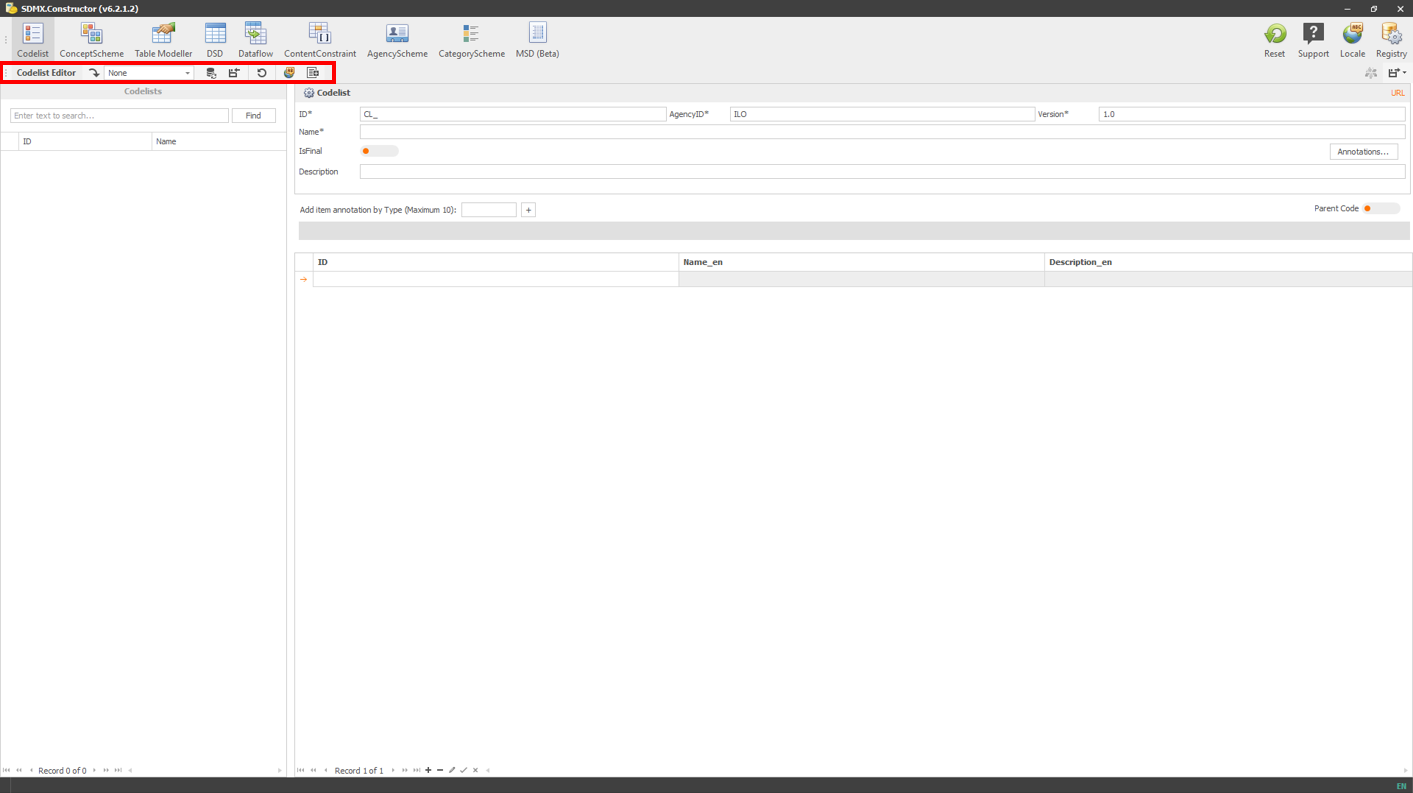
\includegraphics[width=1\linewidth]{./images/image015} \end{center}

\href{images/image015.png}{Click here to enlarge the image}

It contains icons that represent the most commonly used features of the selected options above, and hovering over each icon will reveal a tooltip that describes its function. The options available in this group of menu items change according to the menu item selected on the top menu.

Below are the icons representing the menu items (Editor Ribbon) and their functions. Users can change the size of these icons by right-clicking on any of them, selecting Customize, and selecting the appropriate setting in Options.

table

If a user chooses ``Codelist'' from the top menu, the corresponding menu items in the third group will appear as ``Load from registry'' (from the dropdown menu), ``Refresh the registry'', ``Import'', ``Reset the current Editor inputs'', ``Translation Service'', and ``Bulk load''.

However, suppose a user selects ``ConceptScheme'' from the top menu instead. In that case, the user will see three additional options: ``Add New Concept'', ``Load Concept'', and ``Delete Selected Concepts'' relevant to the chosen menu item at the top, i.e., ``ConceptScheme''.

All options available within this menu group per the item selected on the top menu are listed below.

image

The fourth menu item group (Preview and Export) is in the top right corner and below the first group of menu items (as highlighted below).

image

The options available in this group of menu items are related to the preview and export functionalities of the tool and change according to the menu item selected on the top menu (the second group of menu items (Editors)).

Below are the icons representing the menu items, along with their features. Users can change the size of these icons by right-clicking on any of them, selecting Customize, and selecting the appropriate setting in Options.

table

The following section explains the working area of the tool.

Below the menu items on top, the user interface appears divided into two main parts. First, the left pane on the interface serves as a space to hold the artefacts' list. The other side is designated to showcase relevant details (both sides are highlighted in different colours in the screenshot below). Selecting (by double-clicking) an artefact from the left pane prompts its details to appear on the screen's right-side pane. This layout is available for Codelist, Dataflow and ContentConstraint.

image

For ConceptScheme, Table Modeller, DSD, AgencyScheme, CategoryScheme, and MSD, an additional pane also appears in the user interface (below the placeholder for listing the artefacts - (as heightened below)), which acts as a staging area (or a pool). It becomes a CONCEPTS POOL for ConceptScheme, Table Modeller, DSD and MSD options. And it turns into an AGENCY POOL for AgencyScheme and a CATEGORY POOL for CategoryScheme options.

The users can drag the artefacts back and forth between the pool area and the pane on the right.

image

\hypertarget{input-and-output-methods}{%
\section{Input and output methods}\label{input-and-output-methods}}

\hypertarget{translation}{%
\section{Translation}\label{translation}}

\hypertarget{using-sdmx}{%
\chapter{Using SDMX Constructor}\label{using-sdmx}}

\hypertarget{accessing-sdmx}{%
\section{Accessing SDMX artefacts from SDMX registries}\label{accessing-sdmx}}

\hypertarget{default-sdmx-registries}{%
\subsection{Default SDMX registries}\label{default-sdmx-registries}}

\hypertarget{creating-sdmx}{%
\section{Creating SDMX artefacts from scratch}\label{creating-sdmx}}

\hypertarget{setting-up}{%
\subsection{Setting up a registry as a local folder}\label{setting-up}}

\hypertarget{preparing-inputs}{%
\subsection{Preparing inputs}\label{preparing-inputs}}

\hypertarget{creating-agencyscheme}{%
\subsection{Creating AgencyScheme}\label{creating-agencyscheme}}

\hypertarget{creating-conceptscheme}{%
\subsection{Creating ConceptScheme \& Codelist}\label{creating-conceptscheme}}

\hypertarget{creating-dsd}{%
\subsection{Creating DSD, Dataflow, ContentConstraint and CategoryScheme}\label{creating-dsd}}

\hypertarget{working-with-.stat-suite}{%
\section{Working with .Stat Suite}\label{working-with-.stat-suite}}

\hypertarget{upload-the}{%
\subsection{Uploading XML file to the Data Lifecycle Manager (DLM)}\label{upload-the}}

\hypertarget{connect-to}{%
\subsection{Connect to a new SDMX registry}\label{connect-to}}

\hypertarget{footnotes}{%
\section{Footnotes}\label{footnotes}}

Footnotes are put inside the square brackets after a caret \texttt{\^{}{[}{]}}. Like this one \footnote{This is a footnote.}.

\hypertarget{citations}{%
\section{Citations}\label{citations}}

Reference items in your bibliography file(s) using \texttt{@key}.

For example, we are using the \textbf{bookdown} package \citep{R-bookdown} (check out the last code chunk in index.Rmd to see how this citation key was added) in this sample book, which was built on top of R Markdown and \textbf{knitr} \citep{xie2015} (this citation was added manually in an external file book.bib).
Note that the \texttt{.bib} files need to be listed in the index.Rmd with the YAML \texttt{bibliography} key.

The RStudio Visual Markdown Editor can also make it easier to insert citations: \url{https://rstudio.github.io/visual-markdown-editing/\#/citations}

\hypertarget{special-topics}{%
\chapter{Special Topics}\label{special-topics}}

\hypertarget{annotations}{%
\section{Annotations}\label{annotations}}

\hypertarget{table-modeller}{%
\section{Table Modeller}\label{table-modeller}}

\hypertarget{translations-using-google-apideepl}{%
\section{Translations using Google API/DeepL}\label{translations-using-google-apideepl}}

\hypertarget{equations}{%
\section{Equations}\label{equations}}

Here is an equation.

\begin{equation} 
  f\left(k\right) = \binom{n}{k} p^k\left(1-p\right)^{n-k}
  \label{eq:binom}
\end{equation}

You may refer to using \texttt{\textbackslash{}@ref(eq:binom)}, like see Equation \eqref{eq:binom}.

\hypertarget{theorems-and-proofs}{%
\section{Theorems and proofs}\label{theorems-and-proofs}}

Labeled theorems can be referenced in text using \texttt{\textbackslash{}@ref(thm:tri)}, for example, check out this smart theorem \ref{thm:tri}.

\begin{theorem}
\protect\hypertarget{thm:tri}{}\label{thm:tri}For a right triangle, if \(c\) denotes the \emph{length} of the hypotenuse
and \(a\) and \(b\) denote the lengths of the \textbf{other} two sides, we have
\[a^2 + b^2 = c^2\]
\end{theorem}

Read more here \url{https://bookdown.org/yihui/bookdown/markdown-extensions-by-bookdown.html}.

\hypertarget{callout-blocks}{%
\section{Callout blocks}\label{callout-blocks}}

The R Markdown Cookbook provides more help on how to use custom blocks to design your own callouts: \url{https://bookdown.org/yihui/rmarkdown-cookbook/custom-blocks.html}

\hypertarget{sharing-your-book}{%
\chapter{Sharing your book}\label{sharing-your-book}}

\hypertarget{publishing}{%
\section{Publishing}\label{publishing}}

HTML books can be published online, see: \url{https://bookdown.org/yihui/bookdown/publishing.html}

\hypertarget{pages}{%
\section{404 pages}\label{pages}}

By default, users will be directed to a 404 page if they try to access a webpage that cannot be found. If you'd like to customize your 404 page instead of using the default, you may add either a \texttt{\_404.Rmd} or \texttt{\_404.md} file to your project root and use code and/or Markdown syntax.

\hypertarget{metadata-for-sharing}{%
\section{Metadata for sharing}\label{metadata-for-sharing}}

Bookdown HTML books will provide HTML metadata for social sharing on platforms like Twitter, Facebook, and LinkedIn, using information you provide in the \texttt{index.Rmd} YAML. To setup, set the \texttt{url} for your book and the path to your \texttt{cover-image} file. Your book's \texttt{title} and \texttt{description} are also used.

This \texttt{gitbook} uses the same social sharing data across all chapters in your book- all links shared will look the same.

Specify your book's source repository on GitHub using the \texttt{edit} key under the configuration options in the \texttt{\_output.yml} file, which allows users to suggest an edit by linking to a chapter's source file.

Read more about the features of this output format here:

\url{https://pkgs.rstudio.com/bookdown/reference/gitbook.html}

Or use:

\begin{Shaded}
\begin{Highlighting}[]
\NormalTok{?bookdown}\SpecialCharTok{::}\NormalTok{gitbook}
\end{Highlighting}
\end{Shaded}


  \bibliography{book.bib,packages.bib}

\end{document}
